% Options for packages loaded elsewhere
\PassOptionsToPackage{unicode}{hyperref}
\PassOptionsToPackage{hyphens}{url}
\documentclass[
]{ltjsarticle}
\usepackage{xcolor}
\usepackage[margin=2.5cm]{geometry}
\usepackage{amsmath,amssymb}
\setcounter{secnumdepth}{-\maxdimen} % remove section numbering
\usepackage{iftex}
\ifPDFTeX
  \usepackage[T1]{fontenc}
  \usepackage[utf8]{inputenc}
  \usepackage{textcomp} % provide euro and other symbols
\else % if luatex or xetex
  \usepackage{unicode-math} % this also loads fontspec
  \defaultfontfeatures{Scale=MatchLowercase}
  \defaultfontfeatures[\rmfamily]{Ligatures=TeX,Scale=1}
\fi
\usepackage{lmodern}
\ifPDFTeX\else
  % xetex/luatex font selection
\fi
% Use upquote if available, for straight quotes in verbatim environments
\IfFileExists{upquote.sty}{\usepackage{upquote}}{}
\IfFileExists{microtype.sty}{% use microtype if available
  \usepackage[]{microtype}
  \UseMicrotypeSet[protrusion]{basicmath} % disable protrusion for tt fonts
}{}
\makeatletter
\@ifundefined{KOMAClassName}{% if non-KOMA class
  \IfFileExists{parskip.sty}{%
    \usepackage{parskip}
  }{% else
    \setlength{\parindent}{0pt}
    \setlength{\parskip}{6pt plus 2pt minus 1pt}}
}{% if KOMA class
  \KOMAoptions{parskip=half}}
\makeatother
\usepackage{longtable,booktabs,array}
\newcounter{none} % for unnumbered tables
\usepackage{calc} % for calculating minipage widths
% Correct order of tables after \paragraph or \subparagraph
\usepackage{etoolbox}
\makeatletter
\patchcmd\longtable{\par}{\if@noskipsec\mbox{}\fi\par}{}{}
\makeatother
% Allow footnotes in longtable head/foot
\IfFileExists{footnotehyper.sty}{\usepackage{footnotehyper}}{\usepackage{footnote}}
\makesavenoteenv{longtable}
\usepackage{graphicx}
\makeatletter
\newsavebox\pandoc@box
\newcommand*\pandocbounded[1]{% scales image to fit in text height/width
  \sbox\pandoc@box{#1}%
  \Gscale@div\@tempa{\textheight}{\dimexpr\ht\pandoc@box+\dp\pandoc@box\relax}%
  \Gscale@div\@tempb{\linewidth}{\wd\pandoc@box}%
  \ifdim\@tempb\p@<\@tempa\p@\let\@tempa\@tempb\fi% select the smaller of both
  \ifdim\@tempa\p@<\p@\scalebox{\@tempa}{\usebox\pandoc@box}%
  \else\usebox{\pandoc@box}%
  \fi%
}
% Set default figure placement to htbp
\def\fps@figure{htbp}
\makeatother
\setlength{\emergencystretch}{3em} % prevent overfull lines
\providecommand{\tightlist}{%
  \setlength{\itemsep}{0pt}\setlength{\parskip}{0pt}}
\usepackage[haranoaji]{luatexja-preset}
\usepackage{bookmark}
\IfFileExists{xurl.sty}{\usepackage{xurl}}{} % add URL line breaks if available
\urlstyle{same}
\hypersetup{
  hidelinks,
  pdfcreator={LaTeX via pandoc}}

\author{}
\date{}

\begin{document}

\section{局在奇数倍音光源による二重スリット干渉の思考実験 ―
形の保存は条件付きで脆く、単一波長 N=1
が頑健な特別な場合であること（整列条件・許容帯・off-axis
散乱）}\label{ux5c40ux5728ux5947ux6570ux500dux97f3ux5149ux6e90ux306bux3088ux308bux4e8cux91cdux30b9ux30eaux30c3ux30c8ux5e72ux6e09ux306eux601dux8003ux5b9fux9a13-ux5f62ux306eux4fddux5b58ux306fux6761ux4ef6ux4ed8ux304dux3067ux8106ux304fux5358ux4e00ux6ce2ux9577-n1-ux304cux9811ux5065ux306aux7279ux5225ux306aux5834ux5408ux3067ux3042ux308bux3053ux3068ux6574ux5217ux6761ux4ef6ux8a31ux5bb9ux5e2foff-axis-ux6563ux4e71}

\textbf{木原 範昭}

\emph{本稿は\textbf{思考実験（モデル計算）}であり、実測ではない。確立した物理（標準的な波動光学・量子力学）を覆す主張は一切含まない。位置揺らぎをもつ\textbf{局在光源}を二重スリットに通したときの遠方場干渉を、厳密な解析・数値計算によって例示・整理するものである。先行する位置読み出し論文
{[}1{]}
を唯一の自己参照とし、外部引用は確立した教科書事項（空間コヒーレンス／二重スリット遠方場、奇数倍音余弦和の閉形式）に限る。}

バージョン v0.1（2026-06-29） DOI (Version): 10.5281/zenodo.21035831 DOI
(Concept): 10.5281/zenodo.21035830 Zenodo:
https://zenodo.org/records/21035831

\begin{center}\rule{0.5\linewidth}{0.5pt}\end{center}

\subsection{要旨}\label{ux8981ux65e8}

先行論文 {[}1{]} は、\textbf{単一波長}の点光源が位置揺らぎ \(P(y)\)
をもつとき、二重スリット遠方場の各試行で縞が\textbf{同形のまま幾何学的経路差だけシフト}し、反復試行における縞シフト量の分布が
\(P\)
の押し出し（pushforward）として、写像が近軸で線形ゆえ\textbf{形を保つ}こと（\(P=\cos^2\)
なら \(\cos^2\)）を示した。

本稿はこれを、\textbf{局在した光源波}へ拡張する。局在を一定振幅の奇数倍音和（孤立ピーク波
\(S_N\)）で表現し、それを二重スリットに通す。得られる結果は次の三点である。

\begin{enumerate}
\def\labelenumi{\arabic{enumi}.}
\tightlist
\item
  \textbf{形の保存（整列時）}：\(S_N\)
  は奇数倍音の和でありながら、二スリット遠方場で\textbf{形を変えずに}中央に鋭く局在した一本の縞として現れる。ただしこれは光源---スリット間の対角距離
  \(r_k=\sqrt{L^2+(W/2)^2}\) が基本波長 \(\lambda_0\)
  の整数または半整数倍に「整列」する場合に限る：
  \[\sqrt{L^{2}+(W/2)^{2}}=\frac{m}{2}\,\lambda_0\qquad(m\in\mathbb{Z}).\]
\item
  \textbf{鋭敏な整列条件}：整列はナイフエッジではなく幅 \(\sim 1/(2N)\)
  の帯であり、最高奇数倍音次数 \(N\) が大きいほど狭まる。\(\lambda_0\)
  の\textbf{わずかな違い}（本稿の例では約
  \(3\%\)）が、干渉が成立するか散乱するかを分ける。なお\textbf{中央整列の許容帯自体は
  \(W/L\) に依らない}が、\(W/L\) が大きいほど光源が中央を外れたときの
  \textbf{off-axis の脆さ}が増す（§3.3, §4.3）。
\item
  \textbf{2乗確率読み出しの継承と脆さ}：整列した局在光源は、位置揺らぎ下でも縞シフト量の分布が
  \(\cos^2\) をなぞる（{[}1{]} の押し出しを継承）。ただし
  off-axis（\(y\neq0\)）では光源---スリット経路差が左右で不一致になり、局在の整列がわずかに崩れて縞ピークが
  \(\cos^2\) から下方へずれる。このずれは \(|y|\)・\(N\)
  とともに増す。\textbf{単一波長（\(N=1\)）はこの脆さをもたず無条件で}、本稿の手法を
  \(N=1\)・同条件で実行すると {[}1{]} の結果と機械精度で一致する（§5
  で検証）。
\end{enumerate}

\textbf{本稿の正味の新規内容は否定的結果である}：局在化（\(N\ge2\)）は
{[}1{]} の単純明快な押し出しを改善せず、\(N=1\)
にはなかった\textbf{整列拘束}（3.4）と \textbf{off-axis
の脆さ}を加える。形の保存は本物だが\textbf{条件付き・脆く}、\(N=1\)
が頑健な特別な場合である。局在波からボルン統計へ向かう広い枠組みにとっては、この脆さ自体が重要な知見である。これらは新しい確率法則の導出ではなく、入力分布が観測量（縞シフト）へ写される変数変換と、奇数倍音局在波の干渉の整列条件・鋭敏性・脆さの例示である。本稿は思考実験であり、確立した物理を整理するものであって覆すものではない。なお、拡張光源の\textbf{強度積算}による可視度低下（空間コヒーレンス／van
Cittert--Zernike 定理
{[}2,3{]}）は本稿の対象（縞シフトの押し出し）とは別の観測モードである（§6.1）。

\begin{center}\rule{0.5\linewidth}{0.5pt}\end{center}

\subsection{1. はじめに}\label{ux306fux3058ux3081ux306b}

二重スリット干渉は波動光学・量子力学の基本的舞台である。先行論文 {[}1{]}
は、\textbf{位置に揺らぎをもつ静止点光源}（単一波長
\(\lambda_0\)）について、反復観測で縞シフト量にどのような統計が現れるかを問い、次を示した：各試行は同形の縞を幾何学的経路差だけシフトさせ、シフト量は光源位置のほぼ線形な写像であるから、光源位置を分布
\(P(y)\) から反復して引けば、縞シフト量の分布は \(P\)
の押し出しとして近軸で同形を保つ。

本稿はこの設定の光源を、\textbf{局在した波}に置き換える。すなわち、点光源の単一波長
\(\cos\)
ではなく、一定振幅の奇数倍音を重ね合わせて中央に鋭く局在させた波 \(S_N\)
を光源波形とする。問いは二つである：(i)
奇数倍音の和である局在波は、二スリット遠方場で\textbf{形を保って}局在するか、どんな条件で成立するか。(ii)
その局在光源が位置揺らぎをもつとき、{[}1{]} の \(\cos^2\)
読み出しは\textbf{継承されるか、それとも崩れるか}。

幾何配置は {[}1{]} と同一にとる（\(L=10\), \(W=5\), \(\lambda_0\)
は基本波長）。すべては指定した配置の上での厳密計算であり、本稿は思考実験である。記法と余弦和の閉形式は標準的な解析学テキスト
{[}4{]} に、二重スリット遠方場・空間コヒーレンスは標準的な光学テキスト
{[}2,3{]} に従う。

\begin{center}\rule{0.5\linewidth}{0.5pt}\end{center}

\subsection{2.
局在奇数倍音光源}\label{ux5c40ux5728ux5947ux6570ux500dux97f3ux5149ux6e90}

\subsubsection{\texorpdfstring{2.1 孤立ピーク波
\(S_N\)}{2.1 孤立ピーク波 S\_N}}\label{ux5b64ux7acbux30d4ux30fcux30afux6ce2-s_n}

半波長の位相区間 \(\varphi\in[-\pi/2,\pi/2]\)
上で、一定振幅の奇数倍音余弦和を

\[
S_N(\varphi)=\sum_{m=0}^{(N-1)/2}\cos\!\big((2m+1)\varphi\big)
=\frac{\sin\!\big((N+1)\varphi\big)}{2\sin\varphi}
\tag{2.1}
\]

と定義する（\(N\)
は最高奇数倍音次数、奇数。右辺は等差数列の余弦和の閉形式
{[}4{]}）。\(S_N\) は中央 \(\varphi=0\) で主ピーク \(S_N(0)=(N+1)/2\)
をもち、両端 \(\varphi=\pm\pi/2\)
で零となる「孤立ピーク波」である。観測量には非負の二乗振幅 \(|S_N|^2\)
を用い、その中央主ピークの幅は \(1/(N+1)\) のスケールで縮む（図1）。

\begin{figure}
\centering
\pandocbounded{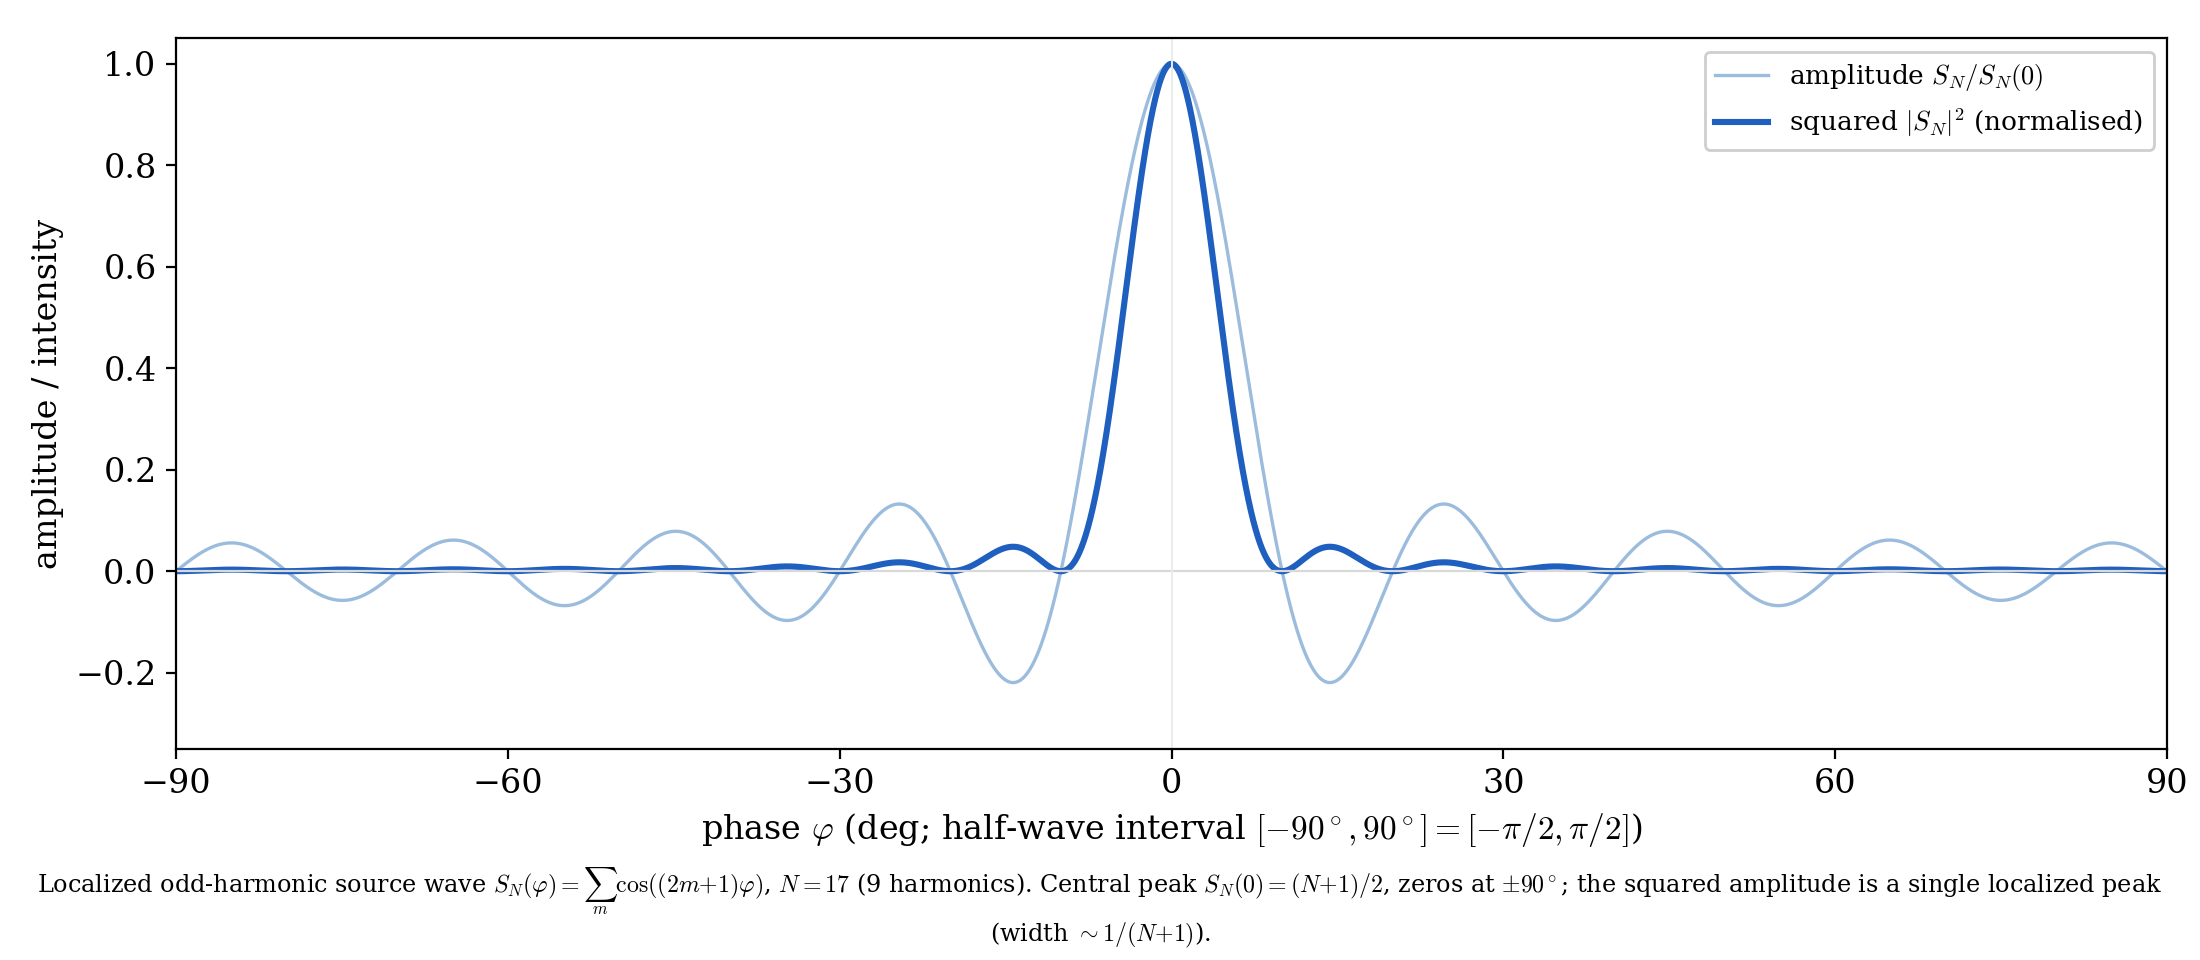
\includegraphics[keepaspectratio,alt={図1 局在奇数倍音光源波 S\_N（N=17）}]{fig_paper2_localized_wave_N17.png}}
\caption{図1 局在奇数倍音光源波 S\_N（N=17）}
\end{figure}

\emph{図1：局在光源波
\(S_N(\varphi)=\sum_m\cos((2m+1)\varphi)\)（\(N=17\)、奇数倍音9本）。薄線は規格化振幅
\(S_N/S_N(0)\)、太線は規格化二乗振幅
\(|S_N|^2\)。中央に単一の鋭い局在ピーク、両端 \(\pm90^\circ\)
で零。基本振動数 \(\nu=1\)・基本波長 \(\lambda_0\)
は奇数倍音で波形を彫っても不変（\(\gcd(1,3,\dots,N)=1\)）。}

\subsubsection{\texorpdfstring{2.2 基本波長
\(\lambda_0\)（檻）と倍音}{2.2 基本波長 \textbackslash lambda\_0（檻）と倍音}}\label{ux57faux672cux6ce2ux9577-lambda_0ux6abbux3068ux500dux97f3}

基本波長 \(\lambda_0\)（最長波長＝\(n=1\)
の波長）を「檻」と呼ぶ。奇数倍音の波長は
\(\lambda_n=\lambda_0/n\)（\(n=1,3,\dots,N\)）であり、\(\lambda_0\)
は局在波の空間周期を与える。\(\nu=1,\lambda_0\)
は相対正規化であり、奇数倍音は局在の鋭さ（相対幅
\(1/(N+1)\)）を変えるのみで基本振動数・基本波長を変えない。

\begin{center}\rule{0.5\linewidth}{0.5pt}\end{center}

\subsection{3.
整列条件と形の保存}\label{ux6574ux5217ux6761ux4ef6ux3068ux5f62ux306eux4fddux5b58}

\subsubsection{3.1
二スリット遠方場（厳密）}\label{ux4e8cux30b9ux30eaux30c3ux30c8ux9060ux65b9ux5834ux53b3ux5bc6}

光源 \(S=(-L,\,y)\)、スリット
\(A_1=(0,+W/2)\)、\(A_2=(0,-W/2)\)。スクリーン点を遠方場回折角
\(\theta_s\)（\(s=\sin\theta_s\)）で表す。波長は全域で各倍音
\(\lambda_n\) 一定（移動仮定もドップラーも導入しない）。各倍音
\(n\)・各アーム \(k\)
の位相は、光源側の幾何学的経路と遠方場のスクリーン側経路差の和

\[
\Phi_k^{(n)}(s;y)=\frac{2\pi n}{\lambda_0}\Big[\,r_k(y)-y_{{\rm slit},k}\,s\,\Big],
\qquad r_k(y)=\sqrt{L^2+(y-y_{{\rm slit},k})^2}
\tag{3.1}
\]

で与えられる（{[}1{]}
の式の倍音版。\(2\pi/\lambda_n=2\pi n/\lambda_0\)）。総複素振幅と強度（複素共役による厳密なボルン形式）は

\[
\psi(s;y)=\sum_{n}\Big[e^{i\Phi_1^{(n)}}+e^{i\Phi_2^{(n)}}\Big],
\qquad I(s;y)=\big|\psi(s;y)\big|^2.
\tag{3.2}
\]

\subsubsection{\texorpdfstring{3.2 中央光源 \(y=0\)
における整列条件}{3.2 中央光源 y=0 における整列条件}}\label{ux4e2dux592eux5149ux6e90-y0-ux306bux304aux3051ux308bux6574ux5217ux6761ux4ef6}

中央光源では \(r_1=r_2=r_k\equiv\sqrt{L^2+(W/2)^2}\) となり、(3.2) は

\[
\psi(s;0)=\sum_n e^{\,i(2\pi n/\lambda_0)\,r_k}\cdot 2\cos\!\Big(\frac{2\pi n}{\lambda_0}\frac{W}{2}\,s\Big)
\tag{3.3}
\]

と書ける。\textbf{光源側位相 \(e^{i(2\pi n/\lambda_0)r_k}\)
は両スリットに共通だが倍音 \(n\) ごとに異なる。} これが全奇数 \(n\)
で揃う（共通因子として括り出せる）条件は、\(2\pi n\,r_k/\lambda_0\) が
\(n\) によらず同一値（mod \(2\pi\)）になること、すなわち

\[
\boxed{\ \frac{r_k}{\lambda_0}=\frac{m}{2}\ \ (m\in\mathbb{Z}),\quad\text{すなわち}\quad
\sqrt{L^{2}+(W/2)^{2}}=\frac{m}{2}\,\lambda_0\ }
\tag{3.4}
\]

である（\(m\) 偶数で位相 \(+1\)、\(m\) 奇数で
\((-1)^n=-1\)、いずれも二乗で同一に整列）。物理的には「光源---スリットの対角距離が基本波長の整数／半整数個ぶん＝スリットが局在波のスパイク（節）に乗る」ことを意味する。

整列するとき (3.3) は
\(\psi(s;0)=({\rm 共通因子})\cdot 2\,S_N(\theta)\)、\(I=4\,S_N(\theta)^2\)（\(\theta=\pi W s/\lambda_0\)）となり、\textbf{スクリーン上の干渉強度が局在波の二乗そのもの}となる。\(|S_N|^2\)
は \(\theta\) について周期 \(180^\circ\)
をもつので、これは厳密には\textbf{周期的な縞列の中央の一本}であり（物理スクリーン
\(|s|\le1\)
には片側に複数本が乗りうる）、その中央が、奇数倍音の和でありながら\textbf{形を変えずに鋭く局在した一本}として現れる（図2）。なお
\(4S_N^2\) は \(\omega,3\omega,5\omega,\dots\)
を位相ロック（周波数コム）した\textbf{瞬時のコヒーレント像}であり、倍音間クロス項を含む。低速検出器による時間平均ではクロス項が落ちて単一倍音縞の和に戻るため、本稿は位相領域の思考実験として瞬時像を扱う。

\begin{figure}
\centering
\pandocbounded{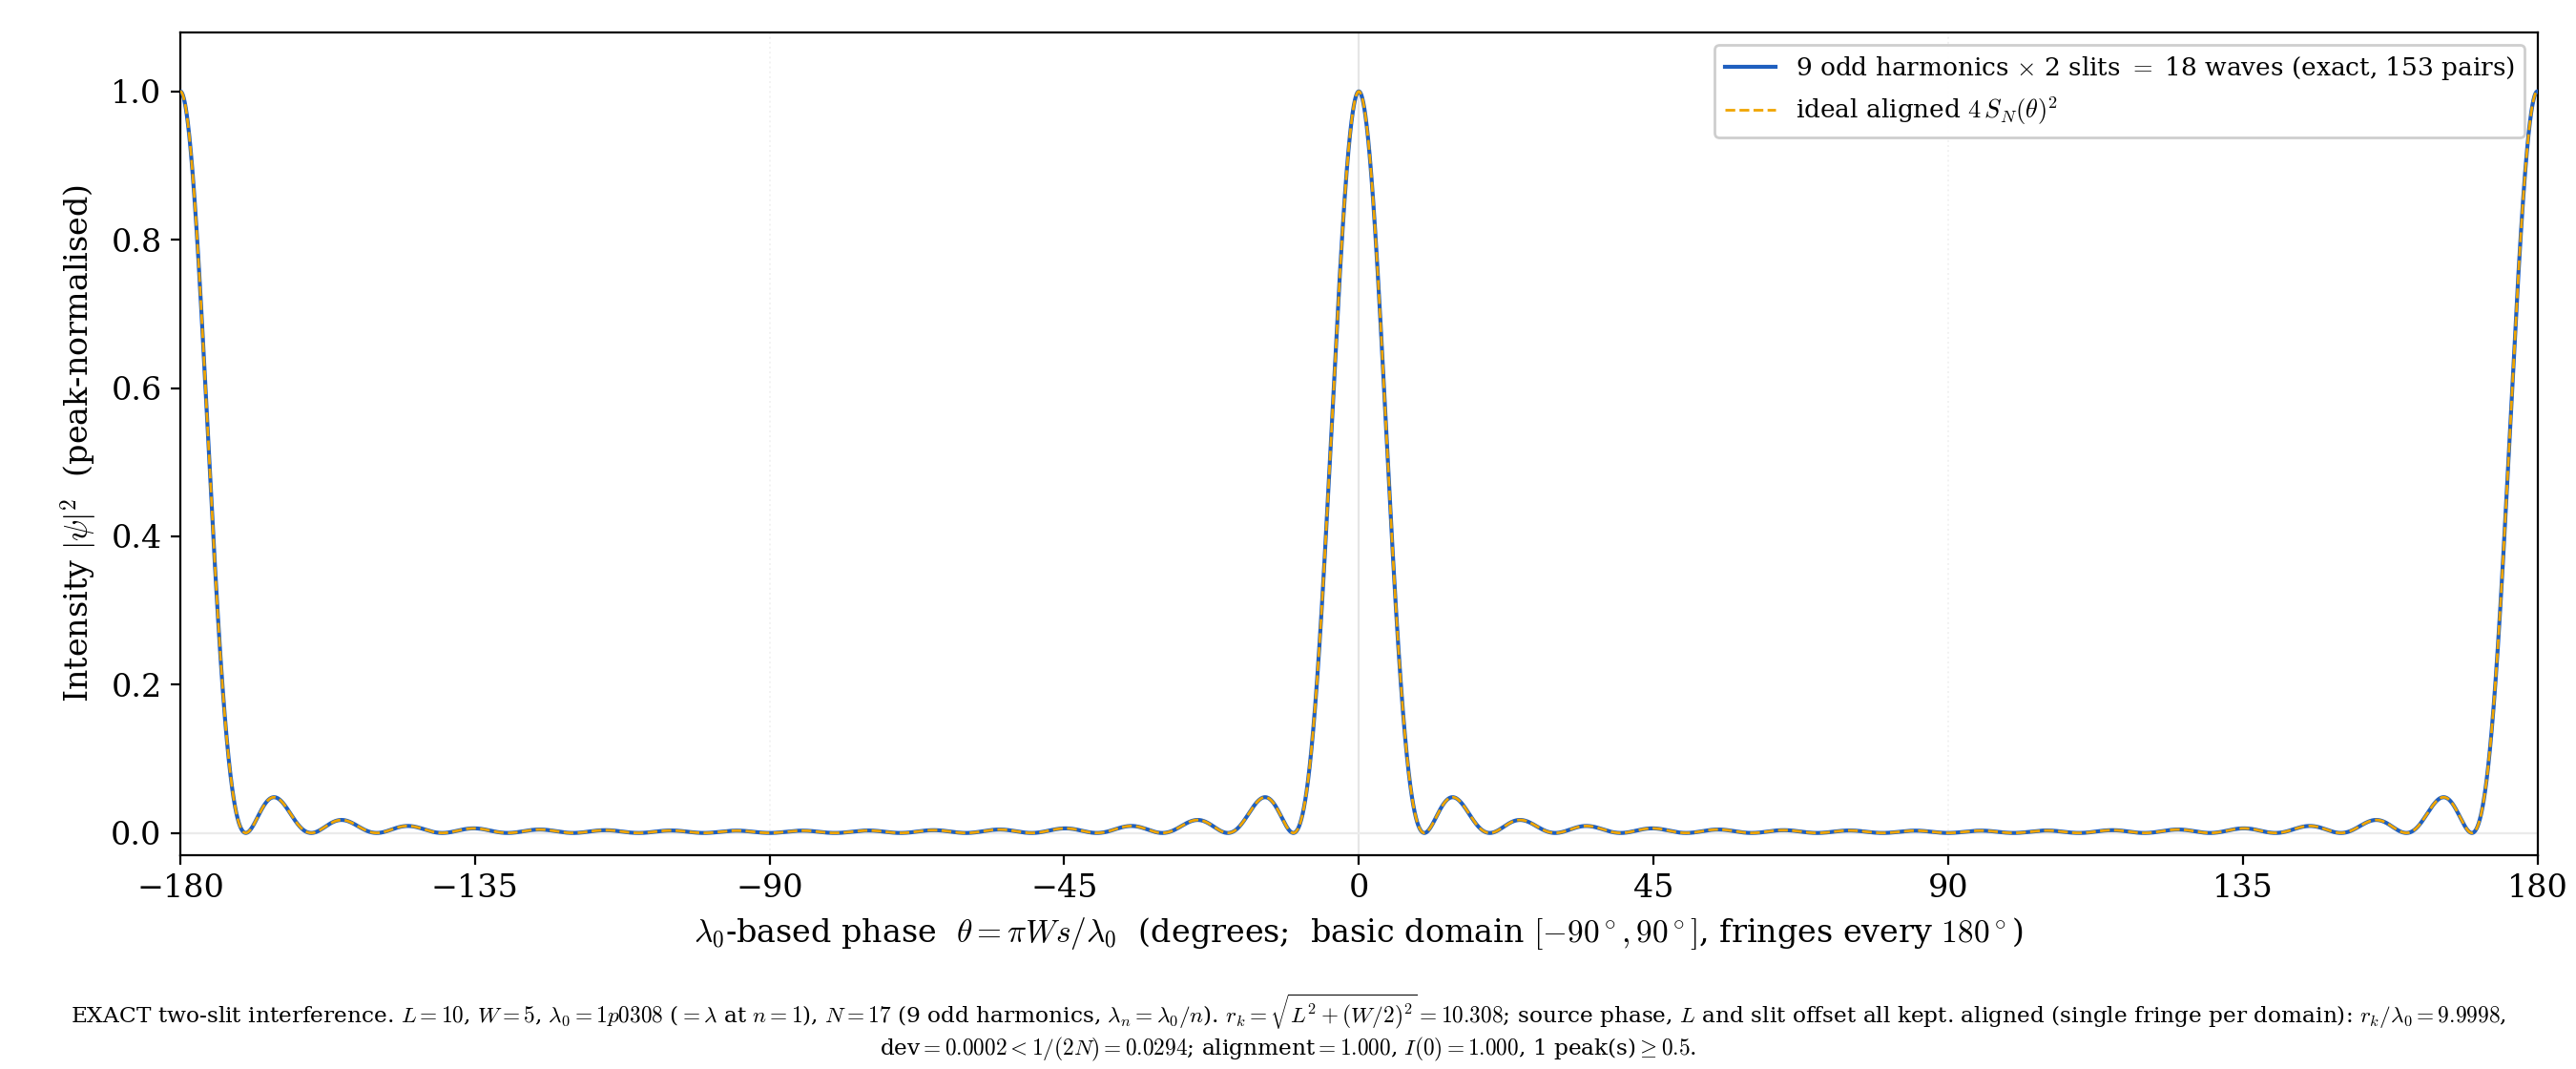
\includegraphics[keepaspectratio,alt={図2 整列した形保存干渉（L=10, W=5, λ0=1.0308, N=17）}]{fig_oddharm_interference_L10_W5_lam1p0308_N17_pm180.png}}
\caption{図2 整列した形保存干渉（L=10, W=5, λ0=1.0308, N=17）}
\end{figure}

\emph{図2：整列した中央光源（\(y=0\)）の二スリット遠方場強度（\(L=10\),
\(W=5\), \(\lambda_0=1.0308\),
\(N=17\)、\(r_k/\lambda_0=10.000\)）。18波（奇数倍音9×2スリット）を厳密に足して二乗。中央に鋭く局在した一本の縞（周期
\(180^\circ\) の縞列の中央。\(|s|\le1\)
には片側に複数本が乗る）、\(I(0)=1\)。破線は理論 \(4S_N(\theta)^2\)
で機械精度一致。横軸は \(\lambda_0\) 基準位相
\(\theta=\pi W s/\lambda_0\)。}

\subsubsection{\texorpdfstring{3.3 鋭敏性：許容帯 \(\sim 1/(2N)\) と
\(W\)
依存の所在}{3.3 鋭敏性：許容帯 \textbackslash sim 1/(2N) と W 依存の所在}}\label{ux92edux654fux6027ux8a31ux5bb9ux5e2f-sim-12n-ux3068-w-ux4f9dux5b58ux306eux6240ux5728}

整列はナイフエッジではなく\textbf{幅のある帯}である。位相誤差は最高倍音で
\(2\pi N\cdot\delta(r_k/\lambda_0)\) と増えるため、許容は

\[
\big|\,r_k/\lambda_0-\tfrac{m}{2}\,\big|\ \lesssim\ \frac{1}{2N}
\tag{3.5}
\]

であり、\(N\) が大きいほど狭い。本稿の幾何（\(L=10\), \(W=5\)）では
\(r_k=\sqrt{106.25}=10.3078\)。\(\lambda_0=1\) なら
\(r_k/\lambda_0=10.308\) で最寄り半整数 \(10.5\) からのずれ
\(0.192\)。これが帯 (3.5) に入るのは
\(N<1/(2\cdot0.192)\approx2.6\)、すなわち\textbf{奇数 \(N\) では \(N=1\)
のみ}。一方
\(\lambda_0=1.0308\)（\(r_k/\lambda_0=10.000\)、\(\lambda_0\) をわずか約
\(3\%\) 変えただけ）なら \(N=17\)（許容
\(\pm0.029\)）でも余裕で整列する。\textbf{\(\lambda_0\)
の僅かな違いが干渉成立／散乱を分ける}。

要求される波長合わせの相対精度は \(\sim 1/(2N\cdot r_k/\lambda_0)\)
のオーダ（\(r_k/\lambda_0\approx10\) なので \(N=17\) で約
\(0.3\%\)、\(N=99\) で約 \(0.05\%\)）。なお、比 \(W/L\)
を固定したまま全体をスケールしても \(r_k/\lambda_0\)
は不変なので、悪い比はスケールでは直らない（\(r_k/L=\sqrt{1+(W/2L)^2}\)
は一般に無理数だが、これは \(W/L\)
の大小によらず成り立つ）。整列を満たすには \(L\) と \(\lambda_0\)
の2自由度を (3.4) に合わせればよい。\textbf{中央整列の許容帯 (3.5)
はそれ自体 \(W/L\) に依らず \(\sim1/(2N)\)} であり、\(W\)
の効果は中央整列ではなく\textbf{光源が中央を外れたとき（off-axis）の脆さ}として現れる（§4.3
で定量する）。

\begin{center}\rule{0.5\linewidth}{0.5pt}\end{center}

\subsection{4.
位置揺らぎ下の2乗確率読み出し}\label{ux4f4dux7f6eux63faux3089ux304eux4e0bux306e2ux4e57ux78baux7387ux8aadux307fux51faux3057}

\subsubsection{4.1 揺らぎの設定（{[}1{]}
と同一）}\label{ux63faux3089ux304eux306eux8a2dux5b9a1-ux3068ux540cux4e00}

光源位置 \(y\) に揺らぎを与え、横方向位置の確率分布を {[}1{]} と同じく

\[
P(y)=\cos^2\!\Big(\frac{\pi y}{\Delta\lambda}\Big),\qquad y\in\Big[-\frac{\Delta\lambda}{2},\,\frac{\Delta\lambda}{2}\Big]
\tag{4.1}
\]

ととる（中央ピーク・端ゼロ。全幅 \(\Delta\lambda\)、半幅
\(\Delta\lambda/2\)。\(\Delta\lambda=\lambda_0\) が {[}1{]} の
\(\pm\lambda/2\) に対応）。光源位置は1試行内で準静的、試行間でこの
\(P(y)\)
に従って引き直されるとする。これまでの実験（\$\S\$3、揺らぎなし）は
\(\Delta\lambda=0\) に相当する。

\begin{figure}
\centering
\pandocbounded{\includegraphics[keepaspectratio,alt={図3 位置揺らぎをもつ光源（{[}1{]} の実験系）}]{fig_setup_source_uncertainty.png}}
\caption{図3 位置揺らぎをもつ光源（{[}1{]} の実験系）}
\end{figure}

\emph{図3：光源---スリット領域の拡大図（{[}1{]} より、\(L=10\),
\(W=5\)）。光源位置は半径 \(\sim\lambda/2\)
の不確定をもち、スクリーンに平行な軸に沿って \(P(y)=\cos^2\)
分布（中央ピーク・端ゼロ）が乗る。本稿はこの光源を局在波 \(S_N\)
に置き換える。}

\subsubsection{4.2
縞シフトの押し出し（厳密計算）}\label{ux7e1eux30b7ux30d5ux30c8ux306eux62bcux3057ux51faux3057ux53b3ux5bc6ux8a08ux7b97}

各光源位置 \(y\) で (3.2) を厳密に計算し（off-axis では
\(r_1(y)\neq r_2(y)\)、光源側位相もすべて保持）、\(P(y)\)
で重み付けし、\(y=0\)
の中央ピーク値で規格化する。局在縞の中央ピークは、全倍音の差位相が揃う
\(\Delta r(y)-Ws=0\) で立ち、その位置は

\[
\Delta r(y)=r_1(y)-r_2(y)\ \approx\ -\frac{W}{L}\,y\ (\text{長さ、近軸で線形}),
\qquad
u(y)=\frac{2\pi}{\lambda_0}\,\Delta r(y)\ \approx\ -\frac{2\pi W}{L\lambda_0}\,y\ (\text{位相})
\tag{4.2}
\]

で与えられ、これは {[}1{]}
の単一波長の縞シフトと同一である。ゆえに縞シフト量の分布は \(P\)
の押し出し \(\rho(u)=P(y(u))|dy/du|\) で、近軸で \(\cos^2\) 形を保つ。

\subsubsection{4.3
結果：継承と脆さ、そして散乱}\label{ux7d50ux679cux7d99ux627fux3068ux8106ux3055ux305dux3057ux3066ux6563ux4e71}

\textbf{(a) \(N=1\)（単一波長、{[}1{]} の再現）.}
倍音は1本だけで、光源側位相 \(e^{i\kappa_1 r_k}\)
は単なる共通の全体位相であり \(|\psi|^2\) で消える。ゆえに整列条件 (3.4)
は\textbf{不要}で、\(L,W,\lambda_0\)
が何であろうと縞は同形でシフトし、ピークが \(\cos^2\)
をなぞる。本稿の手法を \(N=1\)・同条件（\(L=10\), \(W=5\),
\(\lambda_0=1\), \(\Delta\lambda=1\)）で実行すると、{[}1{]}
の図（fig\_decomposition\_static）と\textbf{全数値・全曲線が機械精度（\(\le 2\times10^{-16}\)）で一致}する（§5）。

\begin{figure}
\centering
\pandocbounded{\includegraphics[keepaspectratio,alt={図4 N=1 の位置揺らぎ読み出し（{[}1{]} と機械精度一致）}]{fig_oddharm_fluct_L10_W5_lam1_N1_dlam1.png}}
\caption{図4 N=1 の位置揺らぎ読み出し（{[}1{]} と機械精度一致）}
\end{figure}

\emph{図4：\(N=1\)、\(L=10\), \(W=5\), \(\lambda_0=1\),
\(\Delta\lambda=1\)。各光源
\(y=x\,\Delta\lambda/2\)（\(x\in[-0.8,0.8]\)）の厳密な二スリット強度を
\(P(y)=\cos^2(\pi x/2)\) で重み付けし \(y=0\)
ピークで規格化。縞ピーク（赤）が \(\cos^2\)
押し出し（黄）をなぞる。これは {[}1{]} そのものであり、本稿の基盤が
{[}1{]} と厳密一致することの検証でもある。}

\textbf{(b) \(N=17\)・非整列（\(\lambda_0=1\)）.} §3.3 のとおり
\(\lambda_0=1\) では \(N=17\) は許容帯外で、\textbf{\(y=0\)
の時点で既に局在が立たない}（中央コヒーレンス
\(\approx25\%\)）。縞は二股・多峰に割れ、ピークは \(\cos^2\)
から大きく外れる（図5）。これは揺らぎの効果ではなく、\textbf{整列していない局在源はそもそも干渉して局在しない}ことを示す。

\begin{figure}
\centering
\pandocbounded{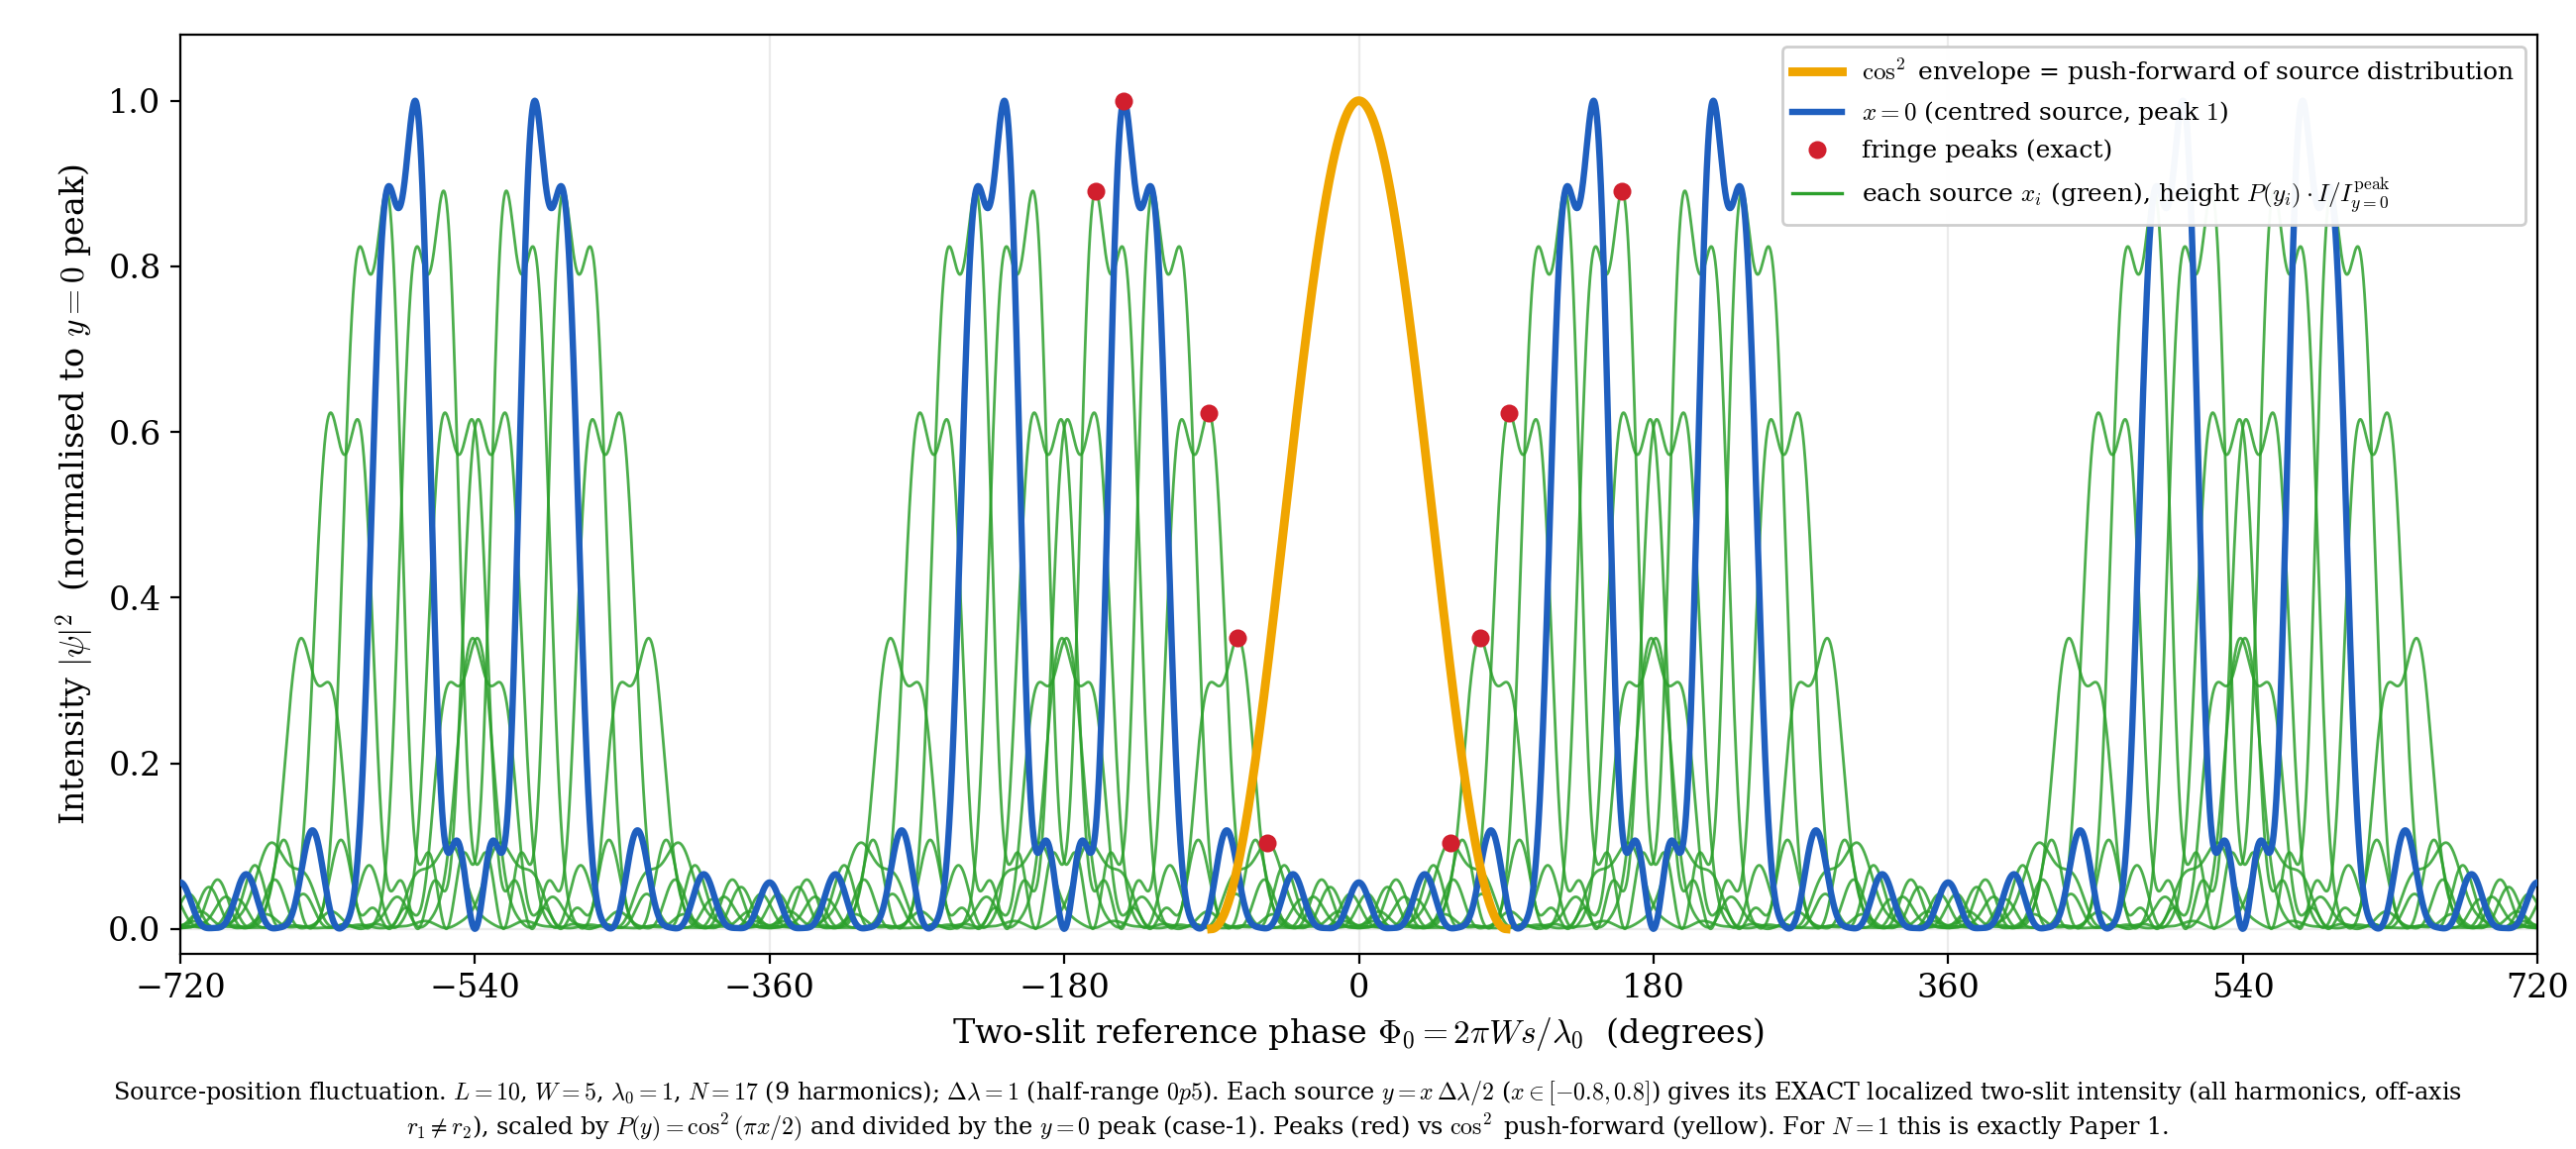
\includegraphics[keepaspectratio,alt={図5 N=17・λ0=1（非整列）：散乱}]{fig_oddharm_fluct_L10_W5_lam1_N17_dlam1.png}}
\caption{図5 N=17・λ0=1（非整列）：散乱}
\end{figure}

\emph{図5：\(N=17\)、\(\lambda_0=1\)（非整列、\(r_k/\lambda_0=10.308\)）。\(y=0\)
でも中央ピーク値は理想 \((N+1)^2\) の約 \(25\%\)
にとどまり、各光源の縞ピークが
\(\cos^2\)（黄）から大きく外れる（散乱）。図4と同一の幾何・揺らぎだが、\(\lambda_0\)
が約 \(3\%\) 違うだけで干渉が崩れる。}

\textbf{(c) \(N=17\)・整列（\(\lambda_0=1.0308\)）.} \(\lambda_0\)
を整列値にすると \(y=0\) で完全コヒーレント（中央
\(=(N+1)^2=324\)）。鋭い局在縞が同形でシフトし、ピークが \(\cos^2\)
を\textbf{ほぼ}なぞる（図6）。ただし off-axis では \(r_1\neq r_2\)
で整列がわずかに崩れ、ピークが \(\cos^2\)
から\textbf{下方へ}ずれる。このずれは異質な二つの寄与に分けられる：

\begin{itemize}
\tightlist
\item
  \textbf{(i) 良性の押し出し非線形性}（全 \(N\) に共通、幾何由来）：写像
  \(u(y)\) の非近軸性によるもので、\(N=1\)
  のずれ（\(-0.0055\!\sim\!-0.027\)）がこれにあたる（{[}1{]} で既出）。
\item
  \textbf{(ii) off-axis 散乱による超過分}（\(N\ge2\)
  で新たに生じる新規部分）：\(y\neq0\) で \(r_1\neq r_2\)
  となり、局在の整列が崩れて局在ピーク自体が低下する。
\end{itemize}

下表で \(N=17\) のずれが \(N=1\) を上回る超過分が、この (ii)
の新規散乱である（厳密には \(N=1\) は \(\lambda_0=1\)、\(N=17\) は
\(\lambda_0=1.0308\) と幾何がわずかに異なり (i)
成分も完全一致ではないが、比較は概ね有効）。例えば
\(x=0.8\)（\(y=0.4\)）でピークは \(P(y)\) の約 \(95\%\)（約 \(5\%\)
の散乱損失）であり、超過分は \(|y|\) とともに増す。

この off-axis 散乱は \(W\) に依存する。中央での経路の偏り速度は
\(\,\big|dr_1/dy\big|_{y=0}=(W/2)/r_k\propto W\,\) なので、\(W\)
が大きいほど光源が中央を外れたとき経路がスパイク（節）から速く離れ、散乱が増す。\textbf{これが
§3.3 で予告した「本当の \(W\) 依存」}であり、中央整列の許容帯（\(W\)
非依存）ではなく off-axis の脆さに現れる。

{\def\LTcaptype{none} % do not increment counter
\begin{longtable}[]{@{}
  >{\raggedleft\arraybackslash}p{(\linewidth - 8\tabcolsep) * \real{0.2000}}
  >{\raggedleft\arraybackslash}p{(\linewidth - 8\tabcolsep) * \real{0.2000}}
  >{\raggedleft\arraybackslash}p{(\linewidth - 8\tabcolsep) * \real{0.2000}}
  >{\raggedleft\arraybackslash}p{(\linewidth - 8\tabcolsep) * \real{0.2000}}
  >{\raggedleft\arraybackslash}p{(\linewidth - 8\tabcolsep) * \real{0.2000}}@{}}
\toprule\noalign{}
\begin{minipage}[b]{\linewidth}\raggedleft
\(x\)
\end{minipage} & \begin{minipage}[b]{\linewidth}\raggedleft
ピーク高さ
\end{minipage} & \begin{minipage}[b]{\linewidth}\raggedleft
\(\cos^2\) 包絡値\(^\dagger\)
\end{minipage} & \begin{minipage}[b]{\linewidth}\raggedleft
ずれ（\(N=17\) 整列）
\end{minipage} & \begin{minipage}[b]{\linewidth}\raggedleft
参考：ずれ（\(N=1\)）
\end{minipage} \\
\midrule\noalign{}
\endhead
\bottomrule\noalign{}
\endlastfoot
0.2 & 0.9045 & 0.9153 & \(-0.011\) & \(-0.0055\) \\
0.4 & 0.6529 & 0.6899 & \(-0.037\) & \(-0.0178\) \\
0.6 & 0.3404 & 0.4001 & \(-0.060\) & \(-0.0271\) \\
0.8 & 0.0909 & 0.1442 & \(-0.053\) & \(-0.0233\) \\
\end{longtable}
}

\(^\dagger\)「\(\cos^2\) 包絡値」は\textbf{ピーク位置 \(p_x\)
での包絡値} \(\cos^2(\pi p_x/180^\circ)\) であって、重み
\(\cos^2(\pi x/2)\) ではない（例：\(x=0.2\) で包絡値 \(0.9153\)、一方
重み \(\cos^2(\pi x/2)=0.9045\)）。表の「ずれ」は \textbf{ピーク高さ
\(-\) 包絡値}（包絡基準）。一方、本文の「\(P(y)\) の約
\(95\%\)（散乱損失 \(5\%\)）」は\textbf{重み \(P(y)\)
基準}で、純粋な散乱寄与 (ii) の指標である。両者は基準が異なる。

\begin{figure}
\centering
\pandocbounded{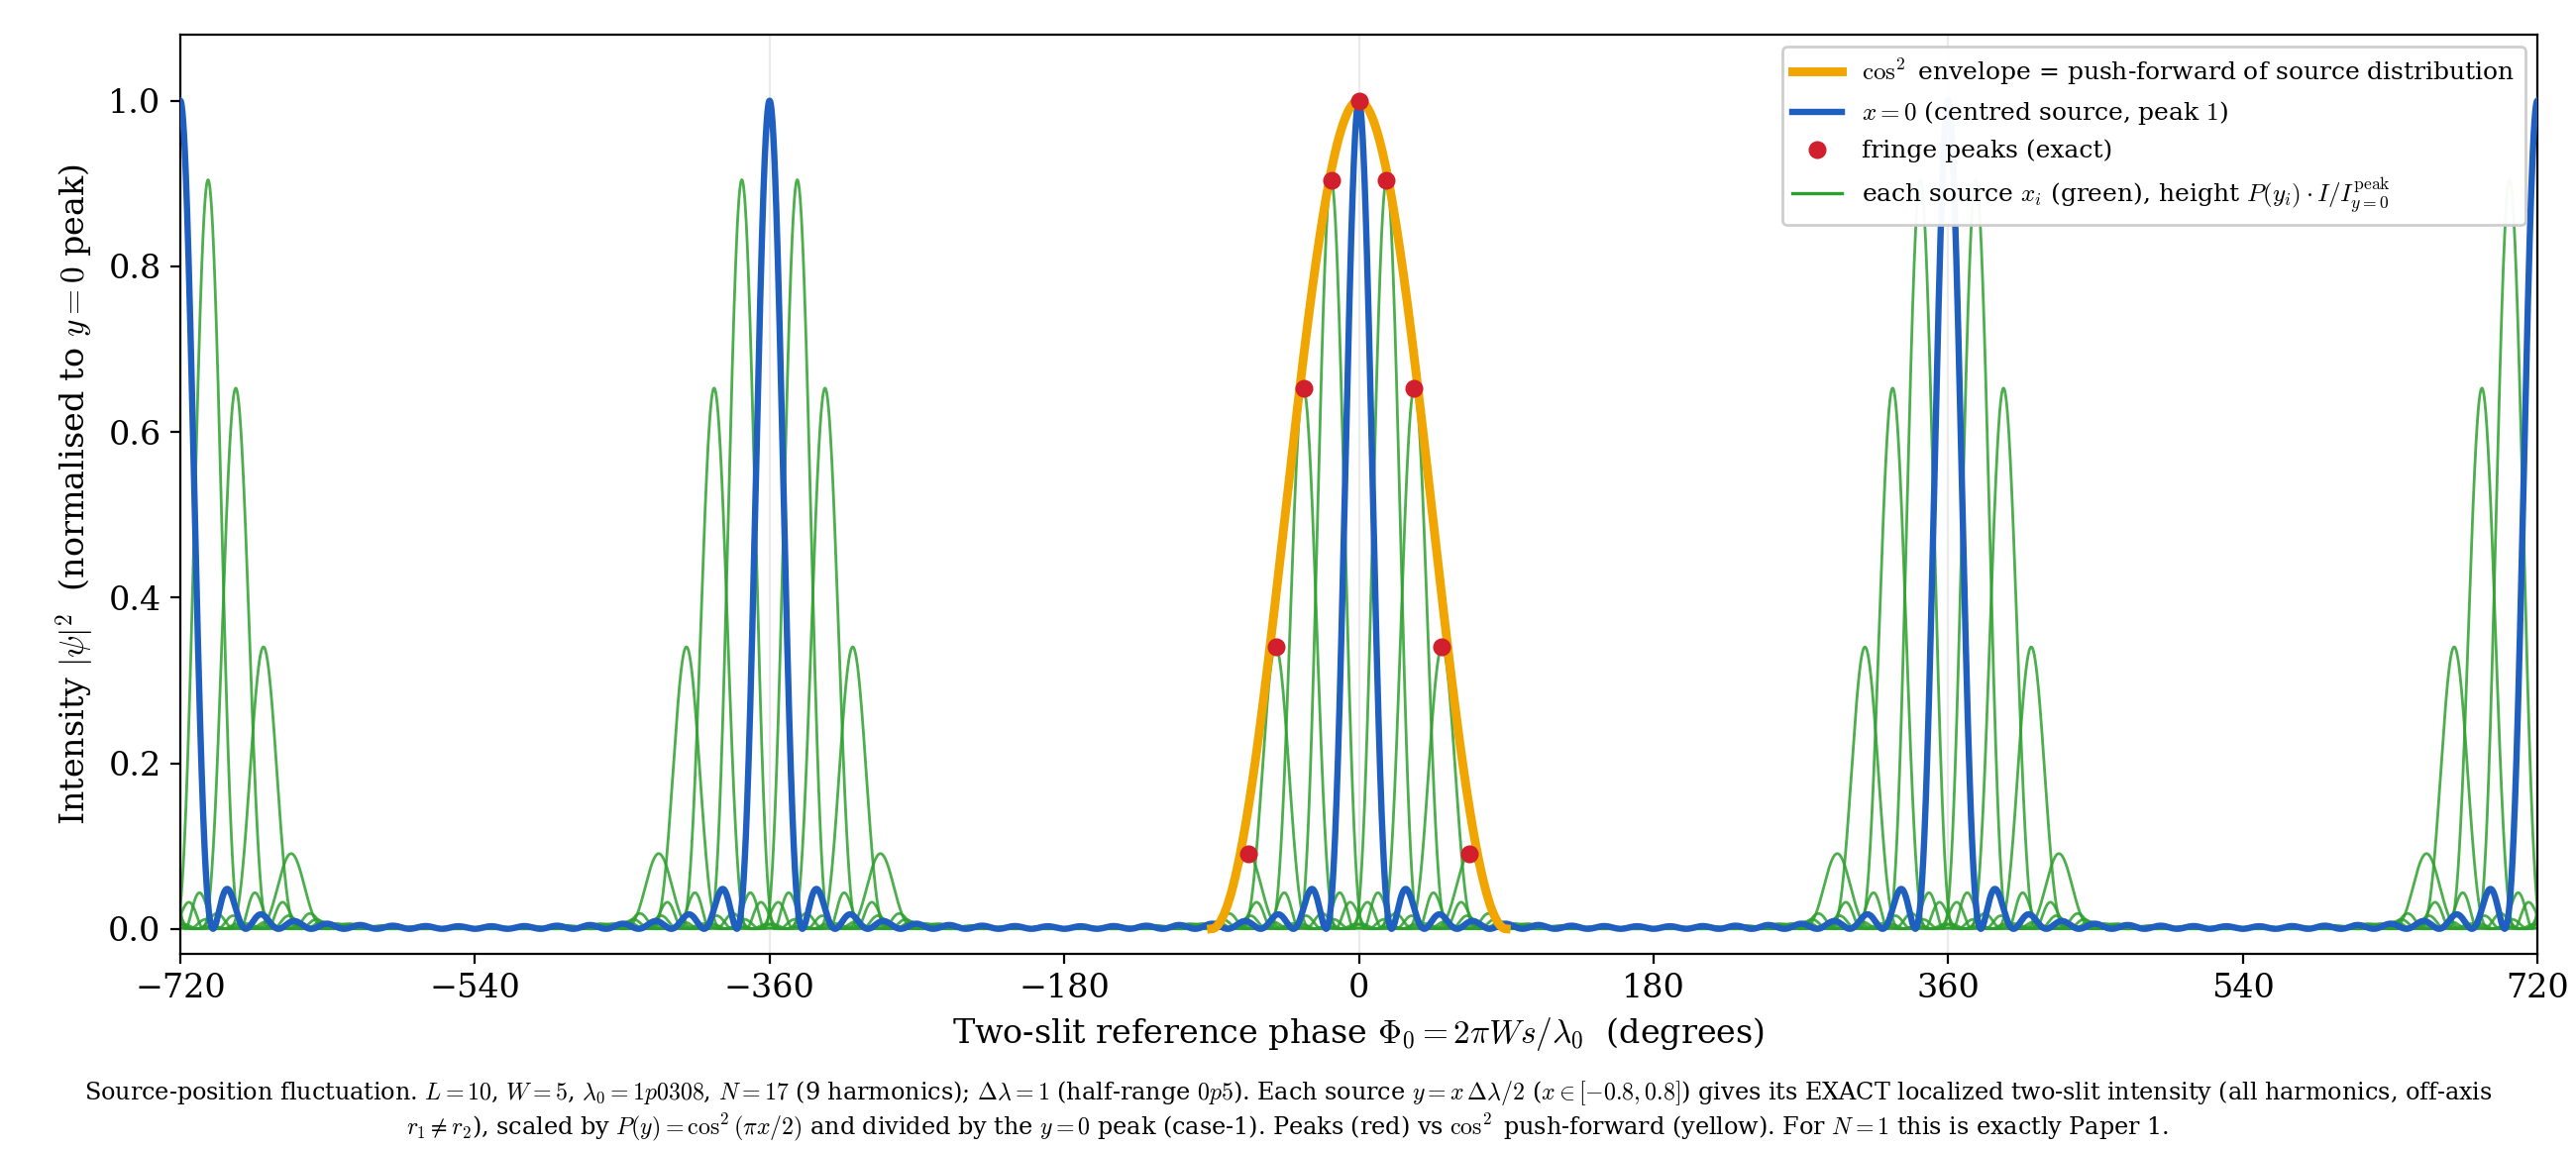
\includegraphics[keepaspectratio,alt={図6 N=17・λ0=1.0308（整列）：cos² をほぼ保つ}]{fig_oddharm_fluct_L10_W5_lam1p0308_N17_dlam1.png}}
\caption{図6 N=17・λ0=1.0308（整列）：cos² をほぼ保つ}
\end{figure}

\emph{図6：\(N=17\)、\(\lambda_0=1.0308\)（整列、\(r_k/\lambda_0=10.000\)）。\(y=0\)
で \(\mathrm{peak}=323.98\approx18^2\)。鋭い局在縞が \(\cos^2\)
包絡（黄）に沿ってシフトし、ピーク（赤）が \(\cos^2\)
をほぼなぞる。off-axis での散乱損失により縁で \(\cos^2\)
より僅かに下方へずれる（上表）。}

\subsubsection{\texorpdfstring{4.4 中央コヒーレンスの \(N\)
依存（\(\lambda_0=1\)）}{4.4 中央コヒーレンスの N 依存（\textbackslash lambda\_0=1）}}\label{ux4e2dux592eux30b3ux30d2ux30fcux30ecux30f3ux30b9ux306e-n-ux4f9dux5b58lambda_01}

\(\lambda_0=1\) における \(y=0\)
の中央コヒーレンス（\(\mathrm{peak}_{y=0}\div\) 理想 \((N+1)^2\)）：

{\def\LTcaptype{none} % do not increment counter
\begin{longtable}[]{@{}rrrrl@{}}
\toprule\noalign{}
\(N\) & \(\mathrm{peak}_{y=0}\) & 理想 \((N+1)^2\) & 整列率 & 判定 \\
\midrule\noalign{}
\endhead
\bottomrule\noalign{}
\endlastfoot
1 & 4.0 & 4 & \(100\%\) & 綺麗 \\
3 & 8.36 & 16 & \(52\%\) & 散乱 \\
5 & 14.97 & 36 & \(42\%\) & 散乱 \\
9 & 27.96 & 100 & \(28\%\) & 散乱 \\
17 & 80.43 & 324 & \(25\%\) & 散乱 \\
\end{longtable}
}

\(\lambda_0=1\) では \(N=1\) のみが整列し、\(N\ge3\)
はすべて散乱する。整列は \(N\) そのものではなく \(r_k/\lambda_0\) が帯
(3.5) に入るかで決まる。

\begin{center}\rule{0.5\linewidth}{0.5pt}\end{center}

\subsection{\texorpdfstring{5. 検証（\(N=1\) で {[}1{]}
と厳密一致）}{5. 検証（N=1 で {[}1{]} と厳密一致）}}\label{ux691cux8a3cn1-ux3067-1-ux3068ux53b3ux5bc6ux4e00ux81f4}

本稿の計算基盤が {[}1{]} と一致することを直接確認した。本稿の手法を
\(N=1\)・\(L=10\), \(W=5\), \(\lambda_0=1\), \(\Delta\lambda=1\)
で実行し（標準プログラム本体を同パラメータで実行）、{[}1{]}
の標準プログラム（fig\_decomposition\_static）の出力と比較したところ：

\begin{itemize}
\tightlist
\item
  9光源点すべてで縞ピーク位置・ピーク高さ・\(\cos^2\)
  値・ずれが\textbf{全行一致}。
\item
  16001点の曲線全体で \textbf{最大絶対差
  \(2.2\times10^{-16}\)}（機械精度）。
\item
  中央 \(y=0\) のピーク値は
  \(4.0\)（\(=2^2\)、二スリットの最大値）で、本稿の「\(y=0\)
  ピーク基準の規格化」が \(N=1\) では {[}1{]}
  の各縞規格化と厳密に等価であることを確認（二スリットのピークは光源位置
  \(y\) に依らず一定だから）。
\end{itemize}

すなわち \(N=1\) は本稿の特別な極限であり、{[}1{]}
はその場合に相当する。

\begin{center}\rule{0.5\linewidth}{0.5pt}\end{center}

\subsection{6. 考察}\label{ux8003ux5bdf}

\subsubsection{6.1 空間コヒーレンス（van
Cittert--Zernike）との区別}\label{ux7a7aux9593ux30b3ux30d2ux30fcux30ecux30f3ux30b9van-cittertzernikeux3068ux306eux533aux5225}

拡張光源・複数光源点からの縞を\textbf{強度で積算}すると、可視度は光源輝度分布のフーリエ変換で与えられ、光源が大きいほど縞が薄れる（空間コヒーレンス、van
Cittert--Zernike 定理 {[}2,3{]}）。これは {[}1{]}
の観測モード(b)（強度積算→可視度低下、入力分布の形にはならない）に対応する確立した結果である。

本稿（および
{[}1{]}）が扱うのは別のモード(a)である：各試行で縞\textbf{シフト量}を読み、反復してヒストグラムを作ると、光源\textbf{位置}分布の押し出しとして\textbf{形が保存}される。可視度低下（モードb／vCZ）と形の保存（モードa／押し出し）は\textbf{別の観測量}であり、混同してはならない。本稿の新規な点は、このモード(a)
を\textbf{局在奇数倍音光源}へ拡張し、形の保存に\textbf{整列条件 (3.4)
と許容帯 \(\sim1/(2N)\)}、すなわち \(\lambda_0\)
の鋭敏性が伴うことを示した点である。これは vCZ にはない側面である。

\subsubsection{6.2
主張の範囲（と非・主張）}\label{ux4e3bux5f35ux306eux7bc4ux56f2ux3068ux975eux4e3bux5f35}

本稿が示したのは次に限る：(i)
局在奇数倍音光源が二スリットで形を保って局在する整列条件 (3.4)
とその鋭敏性 (3.5)；(ii) 整列した局在源は位置揺らぎ下で \(\cos^2\)
読み出しを継承するが、off-axis 散乱で縁が下方へずれること；(iii) \(N=1\)
がこの脆さをもたず {[}1{]}
に厳密一致すること。これらは厳密計算による\textbf{例示・整理}であって、新しい確率法則の導出ではない。\(\cos^2\)（ボルン形）が現れるのは入力
\(P(y)=\cos^2\)
の押し出しであり、確率解釈・二乗則・ランダム性の起源はここでは問わない。「ボルン則の導出」「測定問題の解決」は主張しない。

\subsubsection{6.3
鋭敏性の含意（限定的注記）}\label{ux92edux654fux6027ux306eux542bux610fux9650ux5b9aux7684ux6ce8ux8a18}

\(\lambda_0\)
の僅かな違い（\(\sim 1/(2N)\)）で干渉が成立／散乱に分かれること、\(N\)
が大きい（鋭い局在）ほど要求精度が厳しくなること、そして \(W/L\)
が大きいほど
off-axis（揺らぎ下）の脆さが増すこと（\textbf{中央整列の許容帯自体は
\(W/L\)
に依らない}）は、本稿の幾何配置に対する厳密計算の帰結である。分解能（局在の鋭さ
\(\propto N\)）と頑健性（整列・揺らぎ耐性）のあいだに、\(N\)
で制御されるトレードオフがある。本稿はこの観察以上の物理的解釈を与えない。

\begin{center}\rule{0.5\linewidth}{0.5pt}\end{center}

\subsection{7. 結論}\label{ux7d50ux8ad6}

位置揺らぎをもつ\textbf{局在奇数倍音光源}による二重スリット遠方場干渉について、{[}1{]}
と同一の幾何配置の上で厳密計算により次を示した。

\begin{enumerate}
\def\labelenumi{\arabic{enumi}.}
\tightlist
\item
  局在を奇数倍音和 \(S_N\)
  で表すと、二スリット遠方場で形を保って中央に鋭く局在した一本の縞が得られる。ただし対角距離が基本波長の整数／半整数倍に整列する条件
  \(\sqrt{L^2+(W/2)^2}=(m/2)\lambda_0\) を要する。
\item
  整列は幅 \(\sim1/(2N)\)
  の帯であり、\(N\)（局在の鋭さ）が大きいほど狭い。\(\lambda_0\) の約
  \(3\%\) の違いで干渉成立／散乱が分かれる。中央整列の許容帯自体は
  \(W/L\) に依らないが、\(W/L\) が大きいほど
  off-axis（揺らぎ下）の脆さが増す。
\item
  整列した局在源は位置揺らぎ下でも縞シフト分布が \(\cos^2\)
  をなぞる（{[}1{]} の押し出しを継承）が、off-axis 散乱で縁が \(\cos^2\)
  から下方へずれる。単一波長 \(N=1\)
  はこの脆さをもたず無条件であり、本稿を \(N=1\)・同条件で実行すると
  {[}1{]} と機械精度で一致する。
\end{enumerate}

要するに本稿の正味の知見は、\textbf{局在化（\(N\ge2\)）は {[}1{]}
の押し出しを改善せず、整列拘束と off-axis
脆さを加える}こと、すなわち\textbf{形の保存は条件付き・脆く、\(N=1\)
が頑健な特別な場合}であることである。これは肯定的な「形の保存」よりむしろ、局在化が読み出しを複雑化・脆弱化するという否定的な結果であり、局在波からボルン統計へ向かう枠組みにとってはこの脆さこそが重要な示唆となる。

これは新しい確率法則の導出ではなく、入力分布の押し出し（{[}1{]}）を局在源へ拡張し、その干渉の整列条件・鋭敏性・揺らぎ耐性（とその脆さ）を例示・整理したものである。拡張光源の可視度低下（空間コヒーレンス／vCZ
{[}2,3{]}）とは別の観測モードである。本稿は思考実験であり、確立した物理を整理するものであって覆すものではない。

\begin{center}\rule{0.5\linewidth}{0.5pt}\end{center}

\subsection{参考文献}\label{ux53c2ux8003ux6587ux732e}

{[}1{]} 木原 範昭,
「位置揺らぎを持つ光源による二重スリット干渉の思考実験 ―
光源位置分布の縞シフト量分布への押し出し（形の保存）」, Zenodo, v0.3
(2026), Concept DOI: 10.5281/zenodo.21035808 / Version DOI:
10.5281/zenodo.21035809（本稿の出発点・唯一の自己参照）.

{[}2{]} M. Born and E. Wolf, \emph{Principles of Optics}, 7th (expanded)
ed.~(Cambridge University Press,
1999)（二重スリット遠方場、部分コヒーレンス、van Cittert--Zernike
定理）.

{[}3{]} L. Mandel and E. Wolf, \emph{Optical Coherence and Quantum
Optics} (Cambridge University Press, 1995)（空間コヒーレンスと van
Cittert--Zernike 定理）.

{[}4{]} 高木 貞治, 『解析概論』改訂第3版（岩波書店,
1961）（三角級数、等差数列の余弦和の閉じた形、ディリクレ核）.

\begin{center}\rule{0.5\linewidth}{0.5pt}\end{center}

\subsection{付録：再現コード}\label{ux4ed8ux9332ux518dux73feux30b3ux30fcux30c9}

すべての結果は次の厳密計算スクリプトで再現される（\(\theta\)・経路はすべて
\(L,W,\lambda_0\)
から導出し、定数を恣意的に置かない。移動仮定・ドップラーは用いない）。

\begin{itemize}
\tightlist
\item
  干渉・揺らぎ本体：\texttt{fig\_oddharm\_interference.py}

  \begin{itemize}
  \tightlist
  \item
    整列した形保存干渉（図2）：\texttt{-\/-L\ 10\ -\/-W\ 5\ -\/-lam0\ 1.0308\ -\/-N\ 17\ -\/-halfdeg\ 180}
  \item
    位置揺らぎ読み出し（図4--6）：\texttt{-\/-dlam\ 1}
    を付し、\texttt{-\/-N\ 1}（\(\lambda_0=1\)）／\texttt{-\/-N\ 17}（\(\lambda_0=1\)）／\texttt{-\/-N\ 17\ -\/-lam0\ 1.0308}
  \end{itemize}
\item
  局在光源波 \(S_N\)（図1）：\texttt{make\_paper2\_localized\_wave.py}
\item
  {[}1{]}
  の標準プログラム（検証の基準・図3の系）：\texttt{fig\_decomposition\_static.py},
  \texttt{fig\_setup\_source\_uncertainty.py}
\end{itemize}

揺らぎモードは、各光源 \(y=x\,\Delta\lambda/2\)（\(x\in[-0.8,0.8]\)）で
(3.2)
を全倍音・off-axis（\(r_1\neq r_2\)）・光源側位相込みで厳密計算し、\(P(y)=\cos^2(\pi x/2)\)
で重み付け、\(y=0\) の中央ピークで規格化する（case-1 規格化）。\(N=1\)
ではこれが {[}1{]} と機械精度一致する（§5）。

\end{document}
